203. \begin{figure}[ht!]
\center{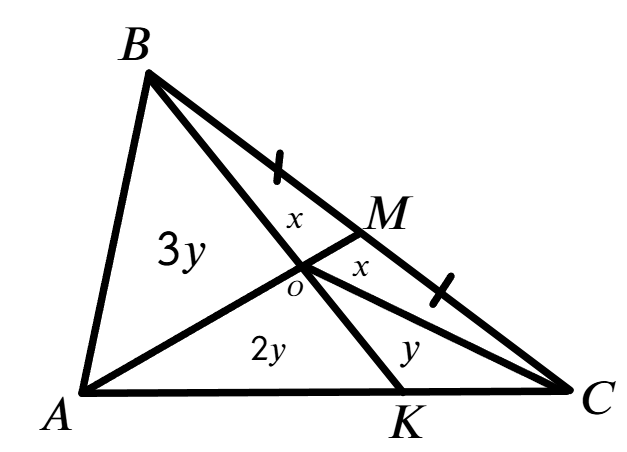
\includegraphics[scale=0.35]{g9-200.png}}
\end{figure}\\
У треугольников, имеющих общую высоту, площади относятся как основания, к которым эта высота проведена, поэтому введём следующие обозначения: $S_{\Delta BOM}=S_{\Delta COM}=x,\ S_{\Delta COK}=y,\ S_{\Delta AOK}=2y.$ Так как $S_{\Delta ABM}=S_{\Delta ACM},$ имеем равенство $S_{\Delta ABO}=2y+y=3y.$
Так как $\cfrac{S_{\Delta ABK}}{S_{\Delta CBK}}=2:1,$ имеем соотношение
$\cfrac{5y}{2x+y}=2,$ откуда $x=\cfrac{3}{4}y.$ Тогда $S=2x+6y=\cfrac{15}{2}y,\ y=\cfrac{2}{15}S,\ x=\cfrac{1}{10}S.$ Таким образом, найдём
$S_{OMCK}=x+y=\cfrac{1}{10}S+\cfrac{2}{15}S=\cfrac{7}{30}S.$\newpage\noindent
